\chapter{Related Work}
\label{ch:RelatedWork}

\section{Sequential left-to-right reduction}
\label{sec:SequentialLeftToRightAddition}


A naive approach to solving above problem is to gather all numbers on a single PE and then apply the reduction
operation strictly from left to right:

\begin{equation}
x_0 \circ x_1 \circ x_2 \circ \ldots  \circ x_{N-1} = ((x_0 \circ x_1) \circ x_2) \circ \ldots
\end{equation}

While simple in implementation, this approach suffers from one major drawback. It does not benefit from any
parallelization whatsoever. Through the communication overhead, performance might actually decrease with
an increasing number of PEs.


\section{Reproducible Accumulators}
\label{sec:Reproducible Accumulators}
For floating-point summation in particular, Ahrens et al. have developed an algorithm that uses a 6-word accumulator
to avoid unpredictable rounding errors \cite{ahrens_algorithms_2020}. After a read-only pass over the input data,
the summation can occur in parallel in no particular order and still produces bitwise identical results.
However, this requires around $9N$ floating-point operations and $3N$ bitwise operations.

Naturally, this approach can not be extended to more general reduction operations, since it depends on specific properties
of floating-point numbers as specified in the IEEE 754 standard \cite{noauthor_ieee_nodate-1}.


\section{Reduction Tree}
\label{sec:ReductionTree}

\begin{figure}
\centering
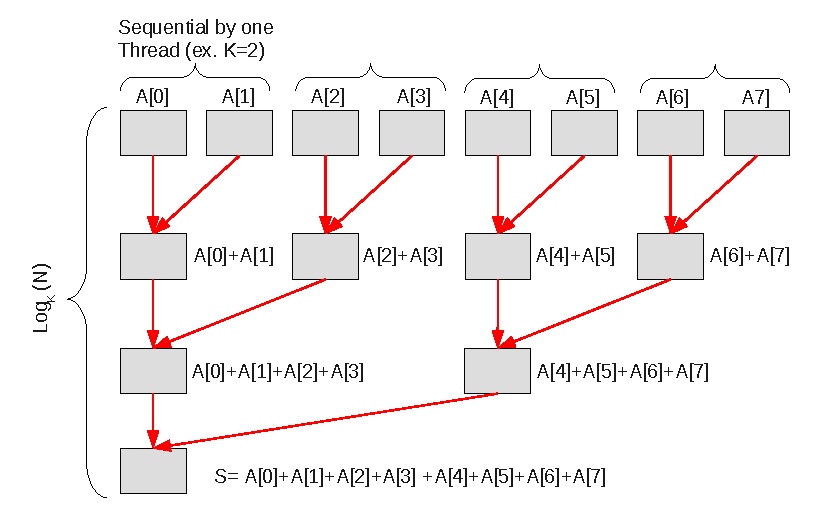
\includegraphics[scale=0.7]{figures/villa_et_al_reduction_tree.pdf}
\caption{Reduction tree. Figure extracted from \cite{villa_effects_2009}}
\label{fig:villa_reduction_tree}
\end{figure}


Villa et al. have utilized a binary tree structure on a Cray XMT system to sum floating-point numbers reproducibly \cite{villa_effects_2009}.
After sequentially summing $K$ elements on each PE, their algorithm uses a parallel-prefix accumulation.
Figure \ref{fig:villa_reduction_tree} gives a schematic overview of the calculation order.

Since the original source code is not available even after contacting the authors, the inner workings of this algorithm are subject to speculation only.

\chapter{Binomial Tree Summation}
\label{ch:BinomialTreeSummation}

\begin{tikzpicture}

\newcommand{\heightFactor}{0.7}
\newcommand{\treeN}{8}
\newcommand{\subtreeHeight}[2]{\directlua{tex.write(subtree_height(#1,#2))}}
\newcommand{\parentIdx}[1]{\directlua{tex.write(parent(#1))}}
\foreach \x in {0,...,\treeN} {
	\node (idx\x{}) at (\x{},0) {\x};
	
	\draw (idx\x{})
		-- (\x{},\heightFactor * \subtreeHeight{\x}{\treeN}+\heightFactor)
		-- (\parentIdx{\x},\heightFactor * \subtreeHeight{\x}{\treeN}+\heightFactor);
}
\end{tikzpicture}